\documentclass{article}
\usepackage[utf8]{inputenc}
\usepackage[includeheadfoot, margin=1em,headheight=2em]{geometry}
\usepackage{titling}
\geometry{a4paper, left=2cm, right=2cm, top=2cm, bottom=2cm}
\usepackage{graphicx}
\usepackage{enumitem}
\usepackage{array}
\usepackage[italian]{babel}
\newcolumntype{P}[1]{>{\centering\arraybackslash}p{#1}}
\renewcommand{\arraystretch}{1.5} % Default value: 1
\setlength{\droptitle}{-6em}

%font
\usepackage[defaultfam,tabular,lining]{montserrat}
\usepackage[T1]{fontenc}
\renewcommand*\oldstylenums[1]{{\fontfamily{Montserrat-TOsF}\selectfont #1}}

%custom bold 
\usepackage[outline]{contour}
\usepackage{xcolor}
\newcommand{\custombold}{\contour{black}}

%table colors
\usepackage{color, colortbl}
\definecolor{Blue}{rgb}{0.51,0.68,0.79}
\definecolor{LightBlue}{rgb}{0.82,0.87,0.90}
\definecolor{LighterBlue}{rgb}{0.93,0.95,0.96}

%Header
\usepackage{fancyhdr, xcolor}
\pagestyle{fancy}
\let\oldheadrule\headrule% Copy \headrule into \oldheadrule
\renewcommand{\headrule}{\color{Blue}\oldheadrule}% Add colour to \headrule
\renewcommand{\headrulewidth}{0.2em}
\fancyhead[L]{Analisi dei reuiqisiti}
\fancyhead[C]{}
\fancyhead[R]{}


\title{\Huge{\textbf{Analisi dei requisiti}}\vspace{-1em}}

\author{CyberSorcerers Team}
\date{}
\begin{document}
\maketitle

\vspace{-3em}
\begin{figure}[h]
  \centering
  
\includegraphics[width=6cm, height=6cm]{documenti/logo rotondo.png}
  \label{fig:immagine}
\end{figure}

\vspace{6em}
\large{

\begin{center}
    \begin{tabular}{l c c}
        \rowcolor{Blue} 
        Informazioni sul documento & &\\ [1 ex]
        \rowcolor{LighterBlue}
        Redattori: &Samuele Vigonotto  &Nicola Lazzarin \\ [1 ex]
        \rowcolor{LightBlue}
        Verificatore:  &  &  \\ [1 ex]
        \rowcolor{LighterBlue}
        Destinatari: & Prf. Tullio Vardanega & Prf. Riccardo Cardin\\ [1 ex]


    \end{tabular}
\end{center}}
\newpage
\custombold{Registro dei Cambiamenti - Changelog}

\begin{center}
\begin{tabular}{P{5em} P{5em} P{8em} P{8em} P{10em}} 
  \rowcolor{Blue}
    \custombold{Versione} & \custombold{Data} & \custombold{Autore} &
    \custombold{ Verificatore} & \custombold{Dettaglio}\\
    \rowcolor{LighterBlue}
     0.0.1& 03/12/2023 & Vignotto Samuele & Lazzarin Nicola & Prima stesura dei casi d'uso e dell'analisi dei requisiti.\\
    \rowcolor{LightBlue}
    0.0.1& 09/12/2023 & Caniato Sabrina  & Vignotto Samuele & Definizione struttura del documento e scheletro delle sezioni. Scrittura introduzione ed obiettivi delle diverse sezioni.\\ 
     & &  &  &\\ 
\end{tabular}
\end{center}
\newpage
\tableofcontents
\section*{Introduzione}

\subsection*{Scopo del documento}

Questo documento ha lo scopo di fornire una descrizione approfondita del prodotto, analizzando nel dettaglio i requisiti, ottenuti tramite incontri con l'azienda e analisi del capitolato. Quest'analisi si concretizza con l'individuazione di casi d'uso, punto centrale di questo documento.


\subsection*{Scopo del prodotto}
L'azienda proponente ha richiesto la creazione di una web app che, tramite l'uso di IA (in questo caso ChatGPT4 e Bedrock) è in grado di creare epic user stories a partire dalle richieste del cliente e confrontarle con il codice sviluppato in modo da informare il cliente dello stato di avanzamento dello sviluppo del prodotto. Inoltre deve essere possibile, sia per il Project Manager, sia per il cliente rilasciare dei feedback (nel primo caso riguardanti l'adeguatezza delle stories,nel secondo caso riguardanti il prodotto finale) al fine di migliorare l'IA. È inoltre richiesta un' analisi comparativa tra le due IA utilizzate e lo sviluppo di un plugin utile agli sviluppatori e al Project Manager.

\subsection*{Glossario}
Alcuni termini presenti nel documento potrebbero essere ambigui, pertanto verranno inseriti nel Glossario v.1.0.0. La loro presenza all'interno di esso sarà indicata tramite una G maiuscola a pedice.

\section*{Casi d'uso}
\subsection*{Scopo}
Lo scopo di questa sezione è raccogliere tutti i casi d'uso individuati, facendo riferimento alle funzionalità individuate durante la sessione di design thinking fatta in collaborazione con l'azienda.

\subsection*{Attori}
Come si è evidenziato durante la sessione di design thinking con i proponenti la web app avrà necessità di tre diverse interfacce per essere usata adeguatamente da tutte le tipologie di attori: clienti, sviluppatori e Project Manager. L'IA (ChatGPT o Bedrock) viene considerata attore secondario in quanto utilizzeremo un servizio che ci viene offerto. Inoltre è necessario lo sviluppo di un plugin accessibile solamente a agli sviluppatori e al Project Manager.\\\\

Per facilitare la comprensione del diagramma dei casi d'uso abbiamo utilizzato due generalizzazioni: Utente e Utente aziendale: 

\begin{figure}[h]
    \centering
    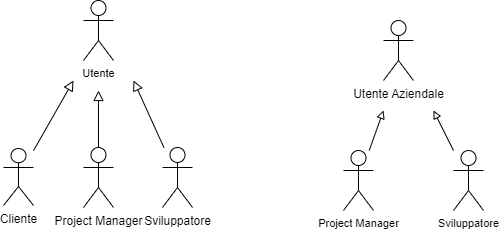
\includegraphics{documenti/imgUML/Attori.png}
    \label{fig:immagine}
\end{figure}

\newpage
\begin{figure}[h]
    \centering
    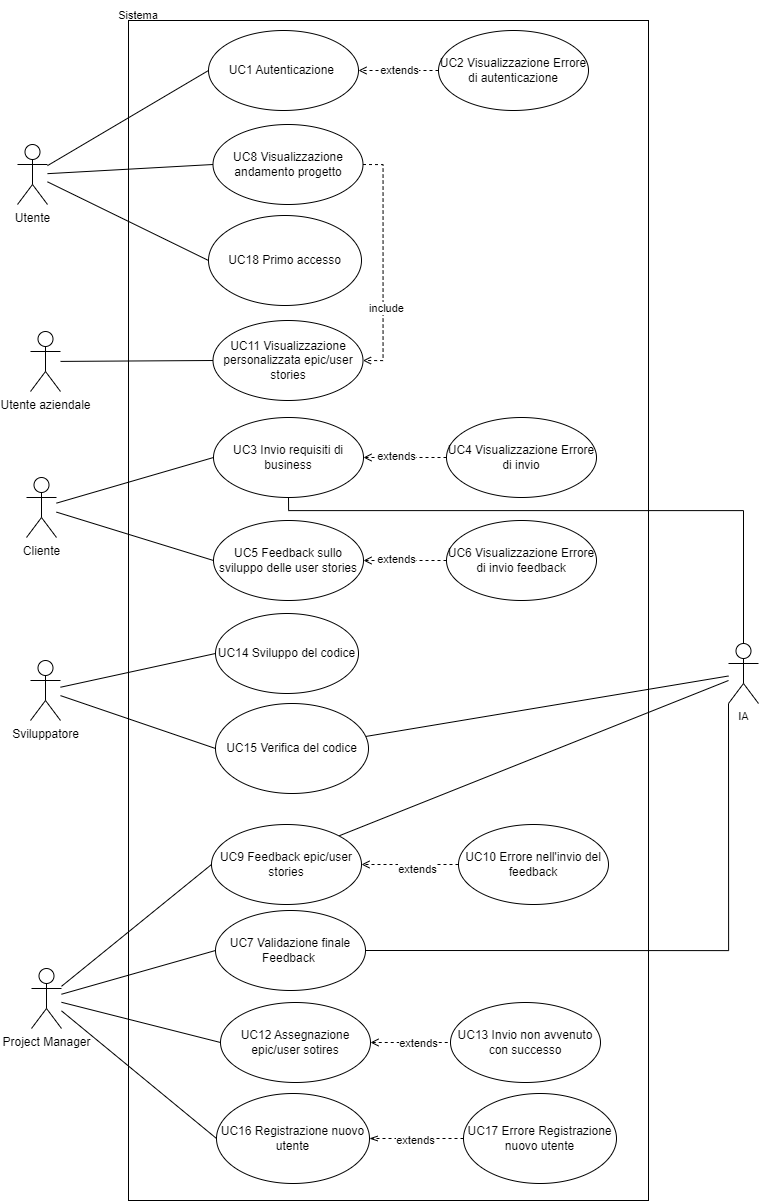
\includegraphics[height = 0.75\textheight]{documenti/imgUML/UML.png}
    \label{fig:immagine}
\end{figure}
\newpage

\section{UC1-Autenticazione}
    \begin{figure}[h]
      \centering
      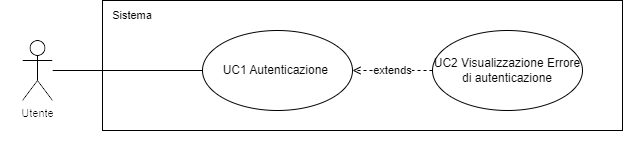
\includegraphics{documenti/imgUML/UC1.png}
      \label{fig:immagine}
    \end{figure} 
    
     \subsection*{Main actor}
         \begin{itemize}
             \item Utente;
         \end{itemize}
     \subsection*{Preconditions} 
        \begin{itemize}
            \item Essere registrati nel sistema con i propri permessi
        \end{itemize}
               
    \subsection*{Postconitions}
        \begin{itemize}
            \item Utente riconosciuto dal sistema;
        \end{itemize}
    \subsection*{Main scenario}
        \begin{figure}[h]
            \centering
            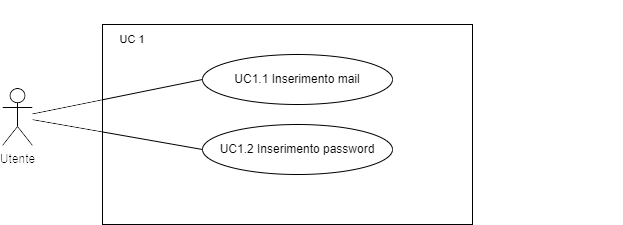
\includegraphics{documenti/imgUML/UC1-zoom.png}
            \label{fig:immagine}
        \end{figure}
            
        \begin{itemize}
            \item Compilazione campo mail [UC1.1];
            \item Compilazione campo password [UC1.2];
        \end{itemize}
            
        \subsection*{Alternative scenario}
            \begin{itemize}
                \item Visualizzazione errore di autenticazione [UC2]
            \end{itemize}
            
\subsection{UC1.1-Inseriemnto Mail}
    
     \subsection*{Main actor}
         \begin{itemize}
             \item Utente;
         \end{itemize}
     \subsection*{Preconditions} 
        \begin{itemize}
            \item Essere registrati nel sistema con i propri permessi
            \item Trovarsi nella pagina di login
        \end{itemize}
        \subsection*{Postcondition} 
        \begin{itemize}
            \item Email inserita
        \end{itemize}

\subsection{UC1.2-Inseriemnto Password}
    
     \subsection*{Main actor}
         \begin{itemize}
             \item Utente;
         \end{itemize}
     \subsection*{Preconditions} 
        \begin{itemize}
            \item Essere registrati nel sistema con i propri permessi
            \item Trovarsi nella pagina di login
        \end{itemize}
        \subsection*{Postcondition} 
        \begin{itemize}
            \item Password inserita
            \item Possibilità di effettuare il login
        \end{itemize}

\section{UC2-Errore di autenticazione}
    
     \subsection*{Main actor}
         \begin{itemize}
             \item Utente;
         \end{itemize}
     \subsection*{Preconditions} 
        \begin{itemize}
            \item Essere registrati nel sistema con i propri permessi
        \end{itemize}
               
    \subsection*{Postconitions}
        \begin{itemize}
            \item Utente Non riconosciuto dal sistema;
        \end{itemize}
            
    
\section{UC3-Compilazione requisiti di business}
    \begin{figure}[h]
      \centering
      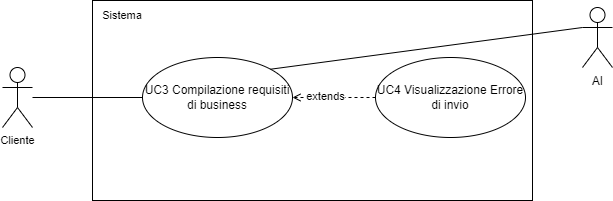
\includegraphics[width=.8\textwidth, height=.6\textheight, keepaspectratio]{documenti/imgUML/UC3.png}
      \label{fig:immagine}
    \end{figure}
     \subsection*{Main actor}
     \begin{itemize}
         \item Cliente;
     \end{itemize}
      \subsection*{Second actor}
     \begin{itemize}
         \item Intelligenza Artificiale;
     \end{itemize}
     \subsection*{Preconditions} 
     \begin{itemize}
         \item Essere riconosciuti dal sistema come Cliente;
         \item Trovarsi nella sezione per aggiungere un nuovo requisito di business
     \end{itemize}
     \subsection*{Postconitions} 
        \begin{itemize}
            \item Invio dei requisiti di business all'intelligenza artificiale;
        \end{itemize}
        
     \subsection*{Main scenario}

        \begin{itemize}
            \item Stesura dei requisiti richiesti;
        \end{itemize}
     \subsection*{Alternative scenario}
        \begin{itemize}
            \item Messaggio d'errore durante l'invio [UC4]
        \end{itemize}

\section{UC4-Errore nell'invio dei requisiti di business}

     \subsection*{Main actor}
     \begin{itemize}
         \item Cliente;
     \end{itemize}
     \subsection*{Preconditions} 
     \begin{itemize}
         \item Essere riconosciuti dal sistema come Cliente;
         \item Trovarsi nella sezione per aggiungere un nuovo requisito di business
     \end{itemize}
     \subsection*{Postconitions} 
        \begin{itemize}
            \item Invio dei requisiti di business all'intelligenza artificiale non riuscito;
        \end{itemize}


\section{UC5-Feedback cliente sullo sviluppo user stories}
    \begin{figure}[h]
      \centering
      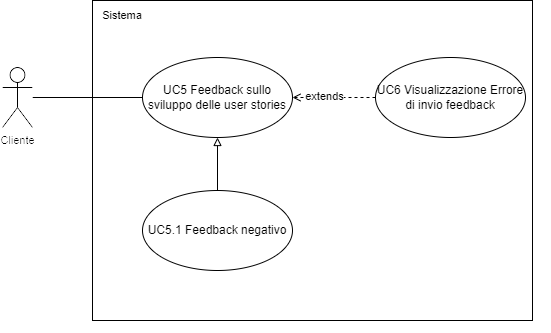
\includegraphics{documenti/imgUML/UC5.png}
      \label{fig:immagine}
    \end{figure}
    
    \subsection*{Main actor}
    \begin{itemize}
        \item Cliente;
    \end{itemize}
    
    \subsection*{Preconditions}
    \begin{itemize}
        \item Essere riconosciuti dal sistema come Cliente;
        \item Presenza di almeno una user story o epic story;
        \item Epic stories completata;
        \item Trovarsi nella user story completata nella sezione apposita per l'invio del feedback;
    \end{itemize}
    
    \subsection*{Postconditions}
    \begin{itemize}
        \item Epic/user stories completato;
    \end{itemize}
    
    \subsection*{Main scenario}
        \begin{figure}[h]
            \centering
            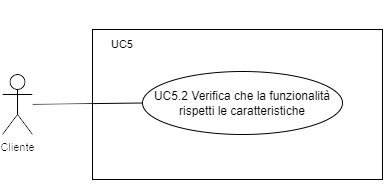
\includegraphics{documenti/imgUML/UC5-zoom.png}
            \label{fig:immagine}
        \end{figure}
        \begin{itemize}
            \item Verifica che la funzionalità rispetti le caratteristiche [UC5.2];
        \end{itemize}
        
    \subsection*{Alternative scenario}
    \begin{itemize}
        \item Visualizazione errore invio feedback[UC6];
    \end{itemize}

    \subsection*{Generalize}
    \begin{figure}[h]
            \centering
            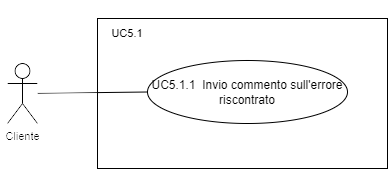
\includegraphics{documenti/imgUML/UC5-zoom1.png}
            \label{fig:immagine}
        \end{figure}
    \subsection{UC5.1 Feedback negativo}
    \begin{itemize}
            \item Invio commento sull'errore riscontrato [UC5.1.1];
        \end{itemize}
        
\section{UC6-Errore nell'invio del feedback}

     \subsection*{Main actor}
     \begin{itemize}
         \item Cliente;
     \end{itemize}
     \subsection*{Preconditions} 
 \begin{itemize}
        \item Essere riconosciuti dal sistema come Cliente;
        \item Presenza di almeno una user story o epic story;
        \item Epic stories completata;
        \item Trovarsi nella user story completata nella sezione apposita per l'invio del feedback;
    \end{itemize}
     \subsection*{Postconitions} 
        \begin{itemize}
            \item Invio del feedback al Project Manager non riuscito;
        \end{itemize} 

        
\section{UC7- Validazione finale del feedback}

\begin{figure}[h]
      \centering
      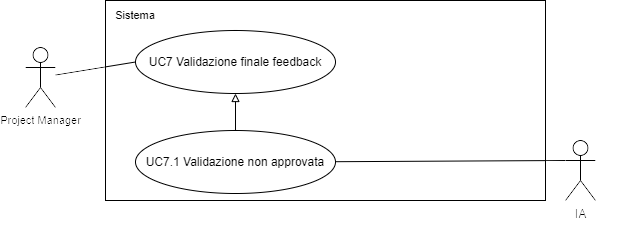
\includegraphics{documenti/imgUML/UC7.png}
      \label{fig:immagine}
    \end{figure}
    
    \subsection*{Main actor}
    \begin{itemize}
        \item Project Manager;
    \end{itemize}
    
    \subsection*{Preconditions}
    \begin{itemize}
        \item Aver ricevuto dal Cliente un feedback negativo riguardante il lavoro finito;
        \item Presenza di almeno una user story o epic story;
        \item Epic stories completata;
    \end{itemize}
    
    \subsection*{Postconditions}
    \begin{itemize}
        \item Epic/user stories completato;
        \item Feedback per epic/user stories ricevuto dal sistema; 
    \end{itemize}
    
    \subsection*{Main scenario}
        \begin{figure}[h]
            \centering
            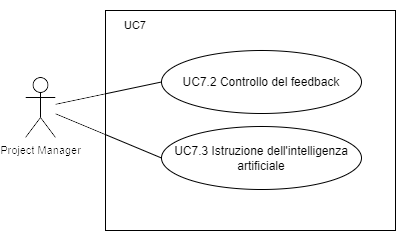
\includegraphics{documenti/imgUML/UC7-zoom.png}
            \label{fig:immagine}
        \end{figure}
        \begin{itemize}
            \item Controllo del feedback inviato [UC7.2];
            \item Istruzione dell'intelligenza artificiale [UC7.3];
        \end{itemize}
        
    \subsection*{Generalize}
      \begin{figure}[h]
            \centering
            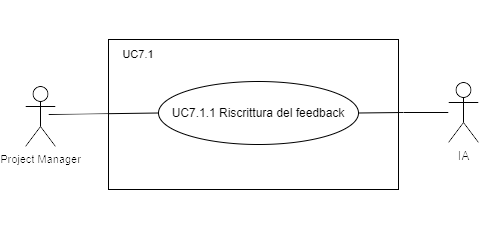
\includegraphics{documenti/imgUML/UC7-zoom1.png}
            \label{fig:immagine}
        \end{figure}
    \subsection{UC7.1 Validazione del feedback non approvata}
    \begin{itemize}
        \item Riscrittura del feedback da parte del Project Manager [UC7.1.1];
        \subsection*{UC7.1.1 Riscrittura del feedback da parte del Project Manager}
     \subsection*{Main actor}
         \begin{itemize}
             \item Project Manager;
         \end{itemize}
     \subsection*{Preconditions} 
        \begin{itemize}
            \item Aver ricevuto un feedback negativo dal cliente;
            \item Il feedback non è comprensibile dall'intelligenza artificiale;
        \end{itemize}
        \subsection*{Postcondition} 
        \begin{itemize}
            \item Il feedback è scritto in modo comprensibile dall'inteligenza artificiale;
        \end{itemize}
    \end{itemize}
    
\subsection{UC7.2-Controllo del feedback inviato}
    
     \subsection*{Main actor}
         \begin{itemize}
             \item Cliente;
         \end{itemize}
     \subsection*{Preconditions} 
        \begin{itemize}
            \item Aver ricevuto un feedback negativo dal cliente;
        \end{itemize}
        \subsection*{Postcondition} 
        \begin{itemize}
            \item Il feedback è scritto in modo comprensibile dall'inteligenza artificiale;
        \end{itemize}
\subsection{UC7.3-Istruzione dell'intelligenza artificiale}
    
     \subsection*{Main actor}
         \begin{itemize}
             \item Cliente;
         \end{itemize}
     \subsection*{Preconditions} 
        \begin{itemize}
            \item Avere un feedback scritto in modo comprensibile dal'intelligenza artificiale;
        \end{itemize}
        \subsection*{Postcondition} 
        \begin{itemize}
            \item L'intelligenza artificiale è stata istruita grazie al feedback ricevuto;
        \end{itemize}

\section{UC8-Visualizzazione andamento progetto}
    \begin{figure}[h]
      \centering
      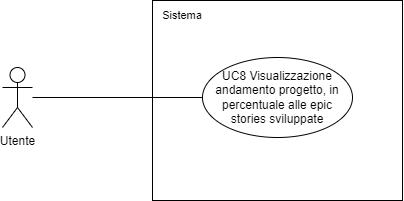
\includegraphics{documenti/imgUML/UC8.png}
      \label{fig:immagine}
    \end{figure}
    
    \subsection*{Main actor}
        \begin{itemize}
            \item Utente; 
        \end{itemize}
        
    \subsection*{Preconditions}
        \begin{itemize}
            \item Essere riconosciuti dal sistema con i propri privilegi;
            \item Cliente ha inviato con successo i requisiti di business al sistema;
            \item Requisiti di business sono stati elaborati dal sistema;
            \item Project Manager ha accettato le epic/user stories generate dal sistema;
            \item Project Manager ha assegnato le epic/user stories agli Sviluppatori;
        \end{itemize}
        
    \subsection*{Postconitions}
        \begin{itemize}
            \item Presa visione dell'andamento del progetto;
        \end{itemize}
        
    \subsection*{Main scenario}
        
        \begin{itemize}
            \item Visualizzazione della percentuale rapprensentante il quantitativo di epic/user stories sviluppate;
        \end{itemize}
        

\section{UC9-Feedback epic/user sotries Project Manager}
    \begin{figure}[h]
      \centering
      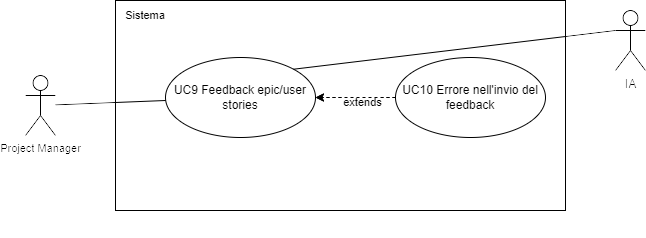
\includegraphics{documenti/imgUML/UC9.png}
      \label{fig:immagine}
    \end{figure}
%con feedback si intende un effetto di reazione prodotto da un messaggio su chi lo ha emesso
    \subsection*{Main actor}
    \begin{itemize}
        \item Project Manager;
    \end{itemize}
    \subsection{Second actor}
    \begin{itemize}
        \item Intelligenza artificiale;
    \end{itemize}
    
    \subsection*{Preconditions}
        \begin{itemize}
            \item Essere riconosciuti dal sistema come Project Manager;
            \item Cliente ha inviato con successo i requisiti di businessa al sistema;
            \item Requisiti di business sono stati elaborati dal sistema;
        \end{itemize}
        
    \subsection*{Postconitions}
        \begin{itemize}
            \item Feedback per epic/user stories ricevuto dal sistema;
            \item Il sistema ha generato epic/user sotries corrette, con corrispettivo tag;
        \end{itemize}
        
    \subsection*{Main scenario}
        \begin{figure}[h]
          \centering
          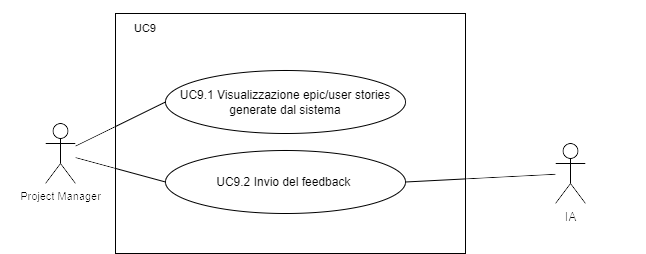
\includegraphics{documenti/imgUML/UC9-zoom.png}
          \label{fig:immagine}
        \end{figure}

        \begin{itemize}
            \item Project Manager visualizza epic/user stories generate dal sistema [UC9.1];
            \item Project Manager invia il feedback al sistema [UC9.2];
        \end{itemize}
        
    \subsection*{Alternative scenario}
        
        \begin{itemize}
            \item Errore nell'invio del feedback[UC10];
        \end{itemize}
        
\section{UC10-Errore nell'invio del feedback}

     \subsection*{Main actor}
     \begin{itemize}
         \item Project Manager;
     \end{itemize}
   \subsection*{Preconditions}
        \begin{itemize}
            \item Essere riconosciuti dal sistema come Project Manager;
            \item Cliente ha inviato con successo i requisiti di businessa al sistema;
            \item Requisiti di business sono stati elaborati dal sistema;
        \end{itemize}
        
    \subsection*{Postconitions}
        \begin{itemize}
            \item Feedback per epic/user stories ricevuto dal sistema;
            \item Il sistema ha generato epic/user sotries corrette, con corrispettivo tag;
        \end{itemize} 

  
\section{UC11-Visualizzazione personalizzata epic/user stories}
    \begin{figure}[h]
      \centering
      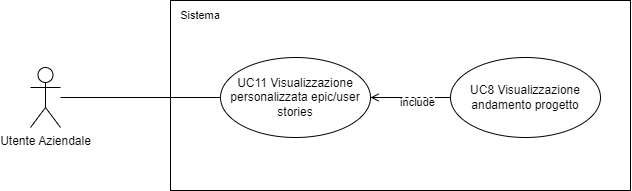
\includegraphics[width=.8\textwidth, height=.6\textheight, keepaspectratio]{documenti/imgUML/UC11.png}
      \label{fig:immagine}
    \end{figure}
    
    \subsection*{Main actor}
        \begin{itemize}
            \item Utente Aziendale;
        \end{itemize}
        
    \subsection*{Preconditions}
        \begin{itemize}
            \item Essere riconosciuti dal sistema con i propri permessi;
            \item Cliente ha inviato con successo i requisiti di businessa al sistema;
            \item requisiti di business sono stati elaborati dal sistema;
            \item Project Manager ha accettato le epic/user stories generate dal sistema;
            \item Project Manager ha assegnato le epic/user stories agli Sviluppatori;
        \end{itemize}
        
    \subsection*{Postconitions}
    \begin{itemize}
        \item Project Manager ha preso visione dell'andamento del progetto;
    \end{itemize}
    
    \subsection*{Main scenario}
        \begin{itemize}
            \item Project Manager visualizza la lista delle epis/user stories assegnate;
        \end{itemize}
        
    \subsection*{Inclusione}
        \begin{itemize}
            \item Visualizzazione andamento progetto [UC8];
        \end{itemize}

\section{UC12-Assegnazione epic/user stories}
    \begin{figure}[h]
      \centering
      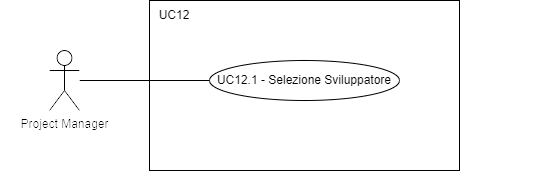
\includegraphics{documenti/imgUML/UC12.png}
      \label{fig:immagine}
    \end{figure}

    \subsection*{Main actor}
    \begin{itemize}
        \item Project Manager;
    \end{itemize}
    
    \subsection*{Preconditions}
        \begin{itemize}
            \item Essere riconosciuto dal sistema come Project Manager;
            \item Le epic/user stories che si vogliono assegnare devono avere feedback positivo;
            \item Trovarsi nella pagina della epic story da assegnare;
        \end{itemize}
        
    \subsection*{Postconditions}
        \begin{itemize}
            \item Una o più epic/user story con feedback positivo è stata assegnata ad uno o più Sviluppatori;
        \end{itemize}
    
    \subsection*{Main scenario}
        \begin{figure}[h]
          \centering
          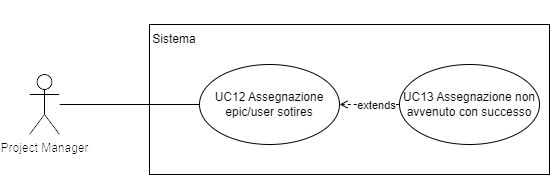
\includegraphics{documenti/imgUML/UC12-zoom.png}
          \label{fig:immagine}
        \end{figure}
        
        \begin{itemize}
            \item Project Manager seleziona lo Sviluppatore a cui assegnare la epic/user story selezionata [UC12.1];
        \end{itemize}
        
    \subsection*{Alternative scenario}
        \begin{itemize}
            \item Errore nell'assegnazione dell'epic story [UC13]
        \end{itemize}    
        
    \subsection{UC12.1- Selezione dello sviluppatore}
        \subsection*{Main actor}
    \begin{itemize}
        \item Project Manager;
    \end{itemize}
    
    \subsection*{Preconditions}
        \begin{itemize}
            \item Essere riconosciuto dal sistema come Project Manager;
            \item Le epic/user stories che si vogliono assegnare devono avere feedback positivo;
            \item Trovarsi nella pagina della epic story da assegnare;
        \end{itemize}
        
    \subsection*{Postconditions}
        \begin{itemize}
            \item Una o più epic/user story con feedback positivo è stata assegnata ad uno o più Sviluppatori;
        \end{itemize}

\section{UC13- Assegnazione non avvenuta}

       \subsection*{Main actor}
    \begin{itemize}
        \item Project Manager;
    \end{itemize}
    
    \subsection*{Preconditions}
        \begin{itemize}
            \item Essere riconosciuto dal sistema come Project Manager;
            \item Le epic/user stories che si vogliono assegnare devono avere feedback positivo;
            \item Trovarsi nella pagina della epic story da assegnare;
        \end{itemize}
        
    \subsection*{Postconditions}
        \begin{itemize}
            \item L'assegnazione non è avvenuta con successo;
        \end{itemize}
    
\section{UC14-Sviluppo del codice}
    \begin{figure}[h]
      \centering
      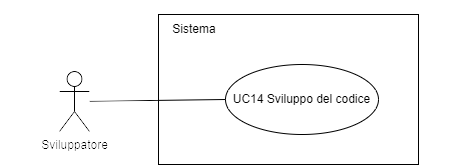
\includegraphics{documenti/imgUML/UC14.png}
      \label{fig:immagine}
    \end{figure}
    
    \subsection*{Main actor}
        \begin{itemize}
            \item Sviluppatore;
        \end{itemize}
    
    \subsection*{Preconditions}
        \begin{itemize}
            \item Essere riconosciuti dal sistema come Sviluppatore;
            \item Avere un'assegnazione per quella user story dal project Managaer;
        \end{itemize}
        
    \subsection*{Postconditions} 
        \begin{itemize}
            \item Il codice svipuppato e pronto per il testing;
            \item Il codice è correttamente taggato;  
        \end{itemize}
    
    \subsection*{Main scenario}
        \begin{figure}[h]
          \centering
          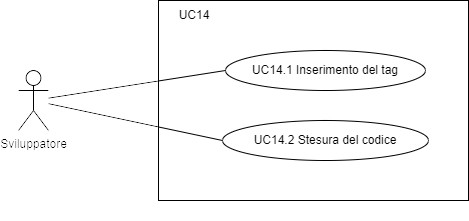
\includegraphics{documenti/imgUML/UC14-zoom.png}
          \label{fig:immagine}
        \end{figure}
        
        \begin{itemize}
            \item Sviluppatore inserisce il tag di riferimento alla user story [UC14.1];
            \item Sviluppatore scrive del codice [UC14.2];
        \end{itemize}

        \subsection{UC14.1 Inserimento del Tag}
\subsection*{Main actor}
        \begin{itemize}
            \item Sviluppatore;
        \end{itemize}
    
    \subsection*{Preconditions}
        \begin{itemize}
            \item Essere riconosciuti dal sistema come Sviluppatore;
            \item Avere un'assegnazione per quella user story dal project Managaer;
        \end{itemize}
        
    \subsection*{Postconditions} 
        \begin{itemize}
            \item Il codice è correttamente taggato;  
        \end{itemize}

        
        \subsection{UC14.2 Stesura del codice}
\subsection*{Main actor}
        \begin{itemize}
            \item Sviluppatore;
        \end{itemize}
    
    \subsection*{Preconditions}
        \begin{itemize}
            \item Essere riconosciuti dal sistema come Sviluppatore;
            \item Avere un'assegnazione per quella user story dal project Managaer;
        \end{itemize}
        
    \subsection*{Postconditions} 
        \begin{itemize}
            \item Il codice svipuppato e pronto per il testing;
        \end{itemize}
        
\section{UC15-Verifica codice da parte dell'AI}
    \begin{figure}[h]
      \centering
      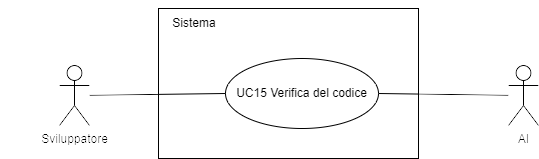
\includegraphics{documenti/imgUML/UC15.png}
      \label{fig:immagine}
    \end{figure}
    
    \subsection*{Main actor}
        \begin{itemize}
            \item Sviluppatore;
        \end{itemize}
    \subsection*{Second actor}
        \begin{itemize}
            \item Intelligenza Artificialie;
        \end{itemize}
    
    \subsection*{Preconditions}
        \begin{itemize}
            \item Essere riconosciuti dal sistema come sviluppatore;
            \item Cliente ha inviato requisiti di business;
            \item Project Manager ha accettato epic/user stories;
            \item Project Manager ha assegnato epic/user stories;
            \item Sviluppatore ha sviluppato codice e test riguardante una o più user story;
            \item Sviluppatore ha taggato correttamente il codice;
        \end{itemize}
        
    \subsection*{Postconditions}
        \begin{itemize}
            \item Sviluppatore riceve feedback da parte del sistema riguardante il codice inviato;
        \end{itemize}
    
    \subsection*{Main scenario}
        \begin{figure}[h]
          \centering
          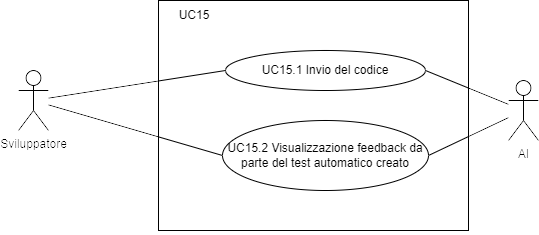
\includegraphics{documenti/imgUML/UC15-zoom.png}
          \label{fig:immagine}
        \end{figure}
        
        \begin{itemize}
            \item Sviluppatore invia codice per la verifica [UC15.1];

            \item Sviluppatore riceve feedback dal sistema riguardante il codice inviato [UC15.2];
        \end{itemize}
        
    \subsection{UC15.1- Invio codice per la verifica}
    \subsection*{Main actor}
        \begin{itemize}
            \item Sviluppatore;
        \end{itemize}
        
    \subsection*{Preconditions}
        \begin{itemize}
            \item Essere riconosciuti dal sistema come sviluppatore;
            \item Cliente ha inviato requisiti di business;
            \item Project Manager ha accettato epic/user stories;
            \item Project Manager ha assegnato epic/user stories;
            \item Sviluppatore ha sviluppato codice e test riguardante una o più user story;
            \item Sviluppatore ha taggato correttamente il codice;
        \end{itemize}
        
    \subsection{UC15.2- Visualizzazione feedback}
    \subsection*{Main actor}
        \begin{itemize}
            \item Sviluppatore;
        \end{itemize}
        
    \subsection*{Preconditions}
        \begin{itemize}
            \item Essere riconosciuti dal sistema come sviluppatore;
            \item Cliente ha inviato requisiti di business;
            \item Project Manager ha accettato epic/user stories;
            \item Project Manager ha assegnato epic/user stories;
            \item Sviluppatore ha sviluppato codice e test riguardante una o più user story;
            \item Sviluppatore ha taggato correttamente il codice;
        \end{itemize}
        
    \subsection*{Postconditions}
        \begin{itemize}
            \item Sviluppatore riceve feedback da parte del sistema riguardante il codice inviato;
            \item Il codice può essere sistemato, in base a quello consigliato dall'intelligenza artificiale;
        \end{itemize}
    

        
\section{UC16-Inserimento di un nuovo cliente}
    \begin{figure}[h]
      \centering
      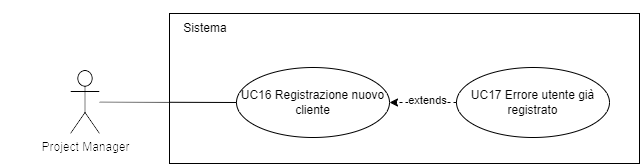
\includegraphics{documenti/imgUML/UC16.png}
      \label{fig:immagine}
    \end{figure}
    
    \subsection*{Main actor}
        \begin{itemize}
            \item Project Manager;
        \end{itemize}
        
    \subsection*{Preconditions}
        \begin{itemize}
            \item Essere riconosciuti dal sistema come Project Manager;
            \item Cliente ha preso contatto con l'azienda per l'inizio di un nuovo progetto insieme;
        \end{itemize}
        
    \subsection*{Postconditions}
        \begin{itemize}
            \item Clienete regisrato nel sistema;
            \item Cliente può effettuare il primo accesso;
        \end{itemize}
    
    \subsection*{Main scenario}
        \begin{figure}[h]
          \centering
          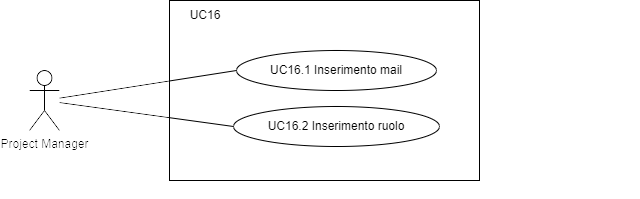
\includegraphics{documenti/imgUML/UC16-zoom.png}
          \label{fig:immagine}
        \end{figure}
        
        \begin{itemize}
            \item Il Project Manager inserisce mail [UC16.1];
            \item Il Project Manager inserisce ruolo di Cliente [UC16.2];
        \end{itemize}
        
    \subsection*{Alternative scenario}
        \begin{itemize}
            \item Errore nella registrazione dell'utente [UC17];
        \end{itemize}

    \subsection{UC16.1- Inserimento Mail}
    \subsection*{Main actor}
        \begin{itemize}
            \item Project Manager;
        \end{itemize}
        
    \subsection*{Preconditions}
        \begin{itemize}
            \item Essere riconosciuti dal sistema come Project Manager;
            \item Cliente ha preso contatto con l'azienda per l'inizio di un nuovo progetto insieme;
        \end{itemize}
        

    \subsection{UC16.2- Inseriemtno ruolo}
    \subsection*{Main actor}
        \begin{itemize}
            \item Project Manager;
        \end{itemize}
        
    \subsection*{Preconditions}
        \begin{itemize}
            \item Essere riconosciuti dal sistema come Project Manager;
            \item Cliente ha preso contatto con l'azienda per l'inizio di un nuovo progetto insieme;
        \end{itemize}
        
    \subsection*{Postconditions}
        \begin{itemize}
            \item Clienete regisrato nel sistema;
            \item Cliente può effettuare il primo accesso;
        \end{itemize}

\section{UC17- Errore nella registrazione dell'utente}
\subsection*{Main actor}
        \begin{itemize}
            \item Project Manager;
        \end{itemize}
        
    \subsection*{Preconditions}
        \begin{itemize}
            \item Essere riconosciuti dal sistema come Project Manager;
            \item Cliente ha preso contatto con l'azienda per l'inizio di un nuovo progetto insieme;
        \end{itemize}
        
    \subsection*{Postconditions}
        \begin{itemize}
            \item Clienete non è regisrato nel sistema;
        \end{itemize}
\section{UC18- Primo accesso}
 \begin{figure}[h]
          \centering
          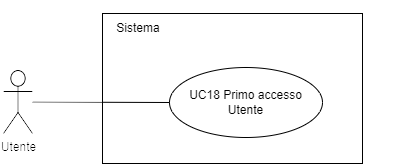
\includegraphics{documenti/imgUML/UC18.png}
          \label{fig:immagine}
        \end{figure}
\subsection*{Main actor}
        \begin{itemize}
            \item Utente;
        \end{itemize}
        
    \subsection*{Preconditions}
        \begin{itemize}
            \item Essere riconosciuti dal sistema con il proprio ruolo;
            \item Non aver ancora effettuato il primo accesso;
        \end{itemize}
        
    \subsection*{Postconditions}
        \begin{itemize}
            \item Clienete regisrato nel sistema con la nuova password;
            \item Cliente può iniziare a scrivere i suoi requisisti di business;
        \end{itemize}
     \subsection*{Main scenario}
        \begin{figure}[h]
          \centering
          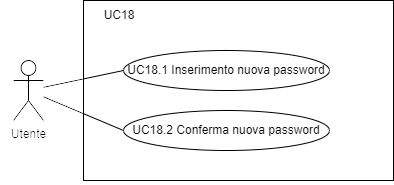
\includegraphics{documenti/imgUML/UC18-zoom.png}
          \label{fig:immagine}
        \end{figure}
        
        \begin{itemize}
            \item Inseriemnto nuova password [UC18.1];
            \item Conferma nuova password [UC18.2];
        \end{itemize}

        \subsection{UC18.1 Inserimento nuova password}
            \subsection*{Main actor}
        \begin{itemize}
            \item Utente;
        \end{itemize}
        
    \subsection*{Preconditions}
        \begin{itemize}
            \item Essere riconosciuti dal sistema con il proprio ruolo;
            \item Non aver ancora effettuato il primo accesso;
        \end{itemize}

    \subsection{UC18.2- Conferma nuova password}
    \subsection*{Main actor}
        \begin{itemize}
            \item Utente;
        \end{itemize}
        
    \subsection*{Preconditions}
        \begin{itemize}
            \item Essere riconosciuti dal sistema con il proprio ruolo;
            \item Non aver ancora effettuato il primo accesso;
        \end{itemize}
        
    \subsection*{Postconditions}
        \begin{itemize}
            \item Clienete regisrato nel sistema con la nuova password;
            \item Cliente può iniziare a scrivere i suoi requisisti di business;
        \end{itemize}

\newpage
\section{Requisiti}
\subsection{Requisiti funzionali}
\begin{center}
    \begin{tabular}{|p{3cm}|p{6cm}|p{3,5cm}|p{3cm}|}
    \rowcolor{Blue} 
\hline
Classificazione & Descrizione & Indirizzato a&Codice  \\ 
\rowcolor{LightBlue}
\hline
Obbligatorio & Accesso a web app tramite login composto da email e password & Sviluppatore, Cliente, Project Manager & UC1, UC16, UC18 \\ 
\rowcolor{LighterBlue}
\hline
Obbligatorio & Scrittura di richieste di buisness tramite box testuale da web app & Cliente & UC3\\ 
\rowcolor{LightBlue}
\hline
Obbligatorio & Invio delle richieste di buisness da web app & Cliente & UC3\\
\hline
\rowcolor{LighterBlue}

Obbligatorio & Visualizzazione andamento sviluppo richieste tramite barra di completamento basata sulla percentuale di user stories completate & Cliente, Project Manager & UC8, UC11\\
\rowcolor{LightBlue}
\hline
Obbligatorio & Approvazione o rifiuto del risultato relativo all'implementazione di una user story & Cliente & UC5\\
\hline
\rowcolor{LighterBlue}

Desiderabile & Ricezione notifiche quando user story completata & Cliente & UC5 UC8\\
\hline
\rowcolor{LightBlue}
\hline
Obbligatorio & Funzionalità di tag nel plugin  & Sviluppatore & UC14\\
\hline
\rowcolor{LighterBlue}

Obbligatorio & Lista di user stories assegnate da Project Manager sia su web app che su plugin & Sviluppatore & UC14 UC15\\
\hline
\rowcolor{LightBlue}

Desiderabile & Ricezione notifica su web app quando nuova users story è assegnata dal Project Manager& Sviluppatore & UC12\\
\hline
\rowcolor{LighterBlue}
Obbligatorio & Invio del codice sviluppato a IA per richiesta verifica& Sviluppatore & UC15\\

\hline
\rowcolor{LightBlue}

Obbligatorio & Visualizzazione users stories generate da IA  & Project Manager & UC9\\
\hline



\end{tabular}

    \begin{tabular}{|p{3cm}|p{6cm}|p{3,5cm}|p{3cm}|}
    \rowcolor{Blue} 
\hline
Classificazione & Descrizione & Indirizzato a&Casi d'uso  \\ 
\rowcolor{LightBlue}
\hline
Obbligatorio & Invio di feedback sulle user stories generate all'IA& Project Manager&UC9\\
\hline
\rowcolor{LighterBlue}

Obbligatorio & Suddivisione delle user stories troppo grandi  & Project Manager& UC9\\
\hline
\rowcolor{LightBlue}

Obbligatorio & Assegnazione user stories agli sviluppatori& Project Manager& UC12\\
\hline
\rowcolor{LighterBlue}

Desiderabile & Ricezione notifiche quando user story viene generata in seguito a richiesta del cliente & Project Manager & UC7\\
\hline
\rowcolor{LightBlue}

Obbligatorio & Invio richiesta di modifiche realtive a user stories a IA prima di approvazione& Project Manager& UC7\\
\hline
\rowcolor{LighterBlue}

Obbligatorio & Visualizzasione andamento epic/user stories assegnate& Sviluppatore& UC11\\

\hline
\end{tabular}
\end{center}

\subsection{Requisiti di qualità}
I requisiti di qualità, e attinenti alle richieste del committente e da lui revisionati,  descrivono le caratteristicge principali e come il sistema deve esibirsi, per soddisfare le esigenze dell'utente.

\begin{center}
    \begin{tabular}{|p{3cm}|p{6cm}|p{3,5cm}|p{3cm}|}
    \rowcolor{Blue} 
\hline
Codice & Descrizione & Fonti  \\ 
\rowcolor{LightBlue}
\hline
& &  \\ 
\rowcolor{LighterBlue}
\hline
 & & \\ 
\rowcolor{LightBlue}
\hline
 & & \\
\hline
\rowcolor{LighterBlue}

& & \\
\rowcolor{LightBlue}
\hline
& & \\
\hline
\rowcolor{LighterBlue}

 & & \\
\hline
\end{tabular}
\end{center}



\subsection{Requisiti di vincolo}
Di seguito la specifica per i requisiti di vincolo, i quali descrivono i limiti e le restrizioni che un sistema
deve rispettare per soddisfare le esigenze dell'utente. 
\begin{center}
    \begin{tabular}{|p{3cm}|p{6cm}|p{3,5cm}|p{3cm}|}
    \rowcolor{Blue} 
\hline
Codice & Descrizione & Fonti  \\ 
\rowcolor{LightBlue}
\hline
& &  \\ 
\rowcolor{LighterBlue}
\hline
 & & \\ 
\rowcolor{LightBlue}
\hline
 & & \\
\hline
\rowcolor{LighterBlue}

& & \\
\rowcolor{LightBlue}
\hline
& & \\
\hline
\rowcolor{LighterBlue}

 & & \\
\hline
\end{tabular}
\end{center}

\subsection{Requisiti sistemi operativi}


\subsection{Requisiti prestazionali}
Per un'applicazione eseguita su una web app, i requisiti prestazionali possono essere influenzati dalle prestazioni del dispositivo dell'utente e la larghezza di banda della connessione Internet 
Non vi sono particolari requisiti in questo senso, in quanto le tecnologie AWS e Chat GPT rispondono in modo ottimale a diverse esigenze:
\begin{itemize}
\item tempo ottimale di risposta;
\item scalabilità, evitando rallentamenti o anomalie non avendo problemi di gestione del carico 
\item utilizzo efficace delle risorse del sistema, riducendo larghezza di banda e non impegnando la memoria del dispositivo, 
\item disponibilità ed affidabilità
\end{itemize}

\subsection{Requisiti di sicurezza}







   
\end{document}
